\documentclass[a4paper]{article}
\usepackage{fullpage} % Smaller margins
\usepackage{graphicx}
\graphicspath{{./images}}

%% Document Header
\title{Weebapedia (working title)}
\author{Alice Charatonik}
\date{}

\begin{document}
\maketitle

\section{Introduction}
An encyclopedia-like database of anime information, moreso focused on answering questions than showing the user all possibly relevant information.

\section{Objectives}
Make it easy for any user to find information about their favorite anime shows or characters, as well as the people and teams who worked on those shows or characters.
\begin{itemize}
  \item Broad questions: eg. "What is Attack on Titan?" or "Who was Satoshi Kon?"
  \item Narrow questions: eg. "Who did Satoshi Kon work with most frequently?"
  \item Relationship questions: eg. "Has Hideaki Anno worked with anyone who would go on to work on Attack on Titan?"
\end{itemize}

\section{Prior Art}
\subsection{MyAnimeList}
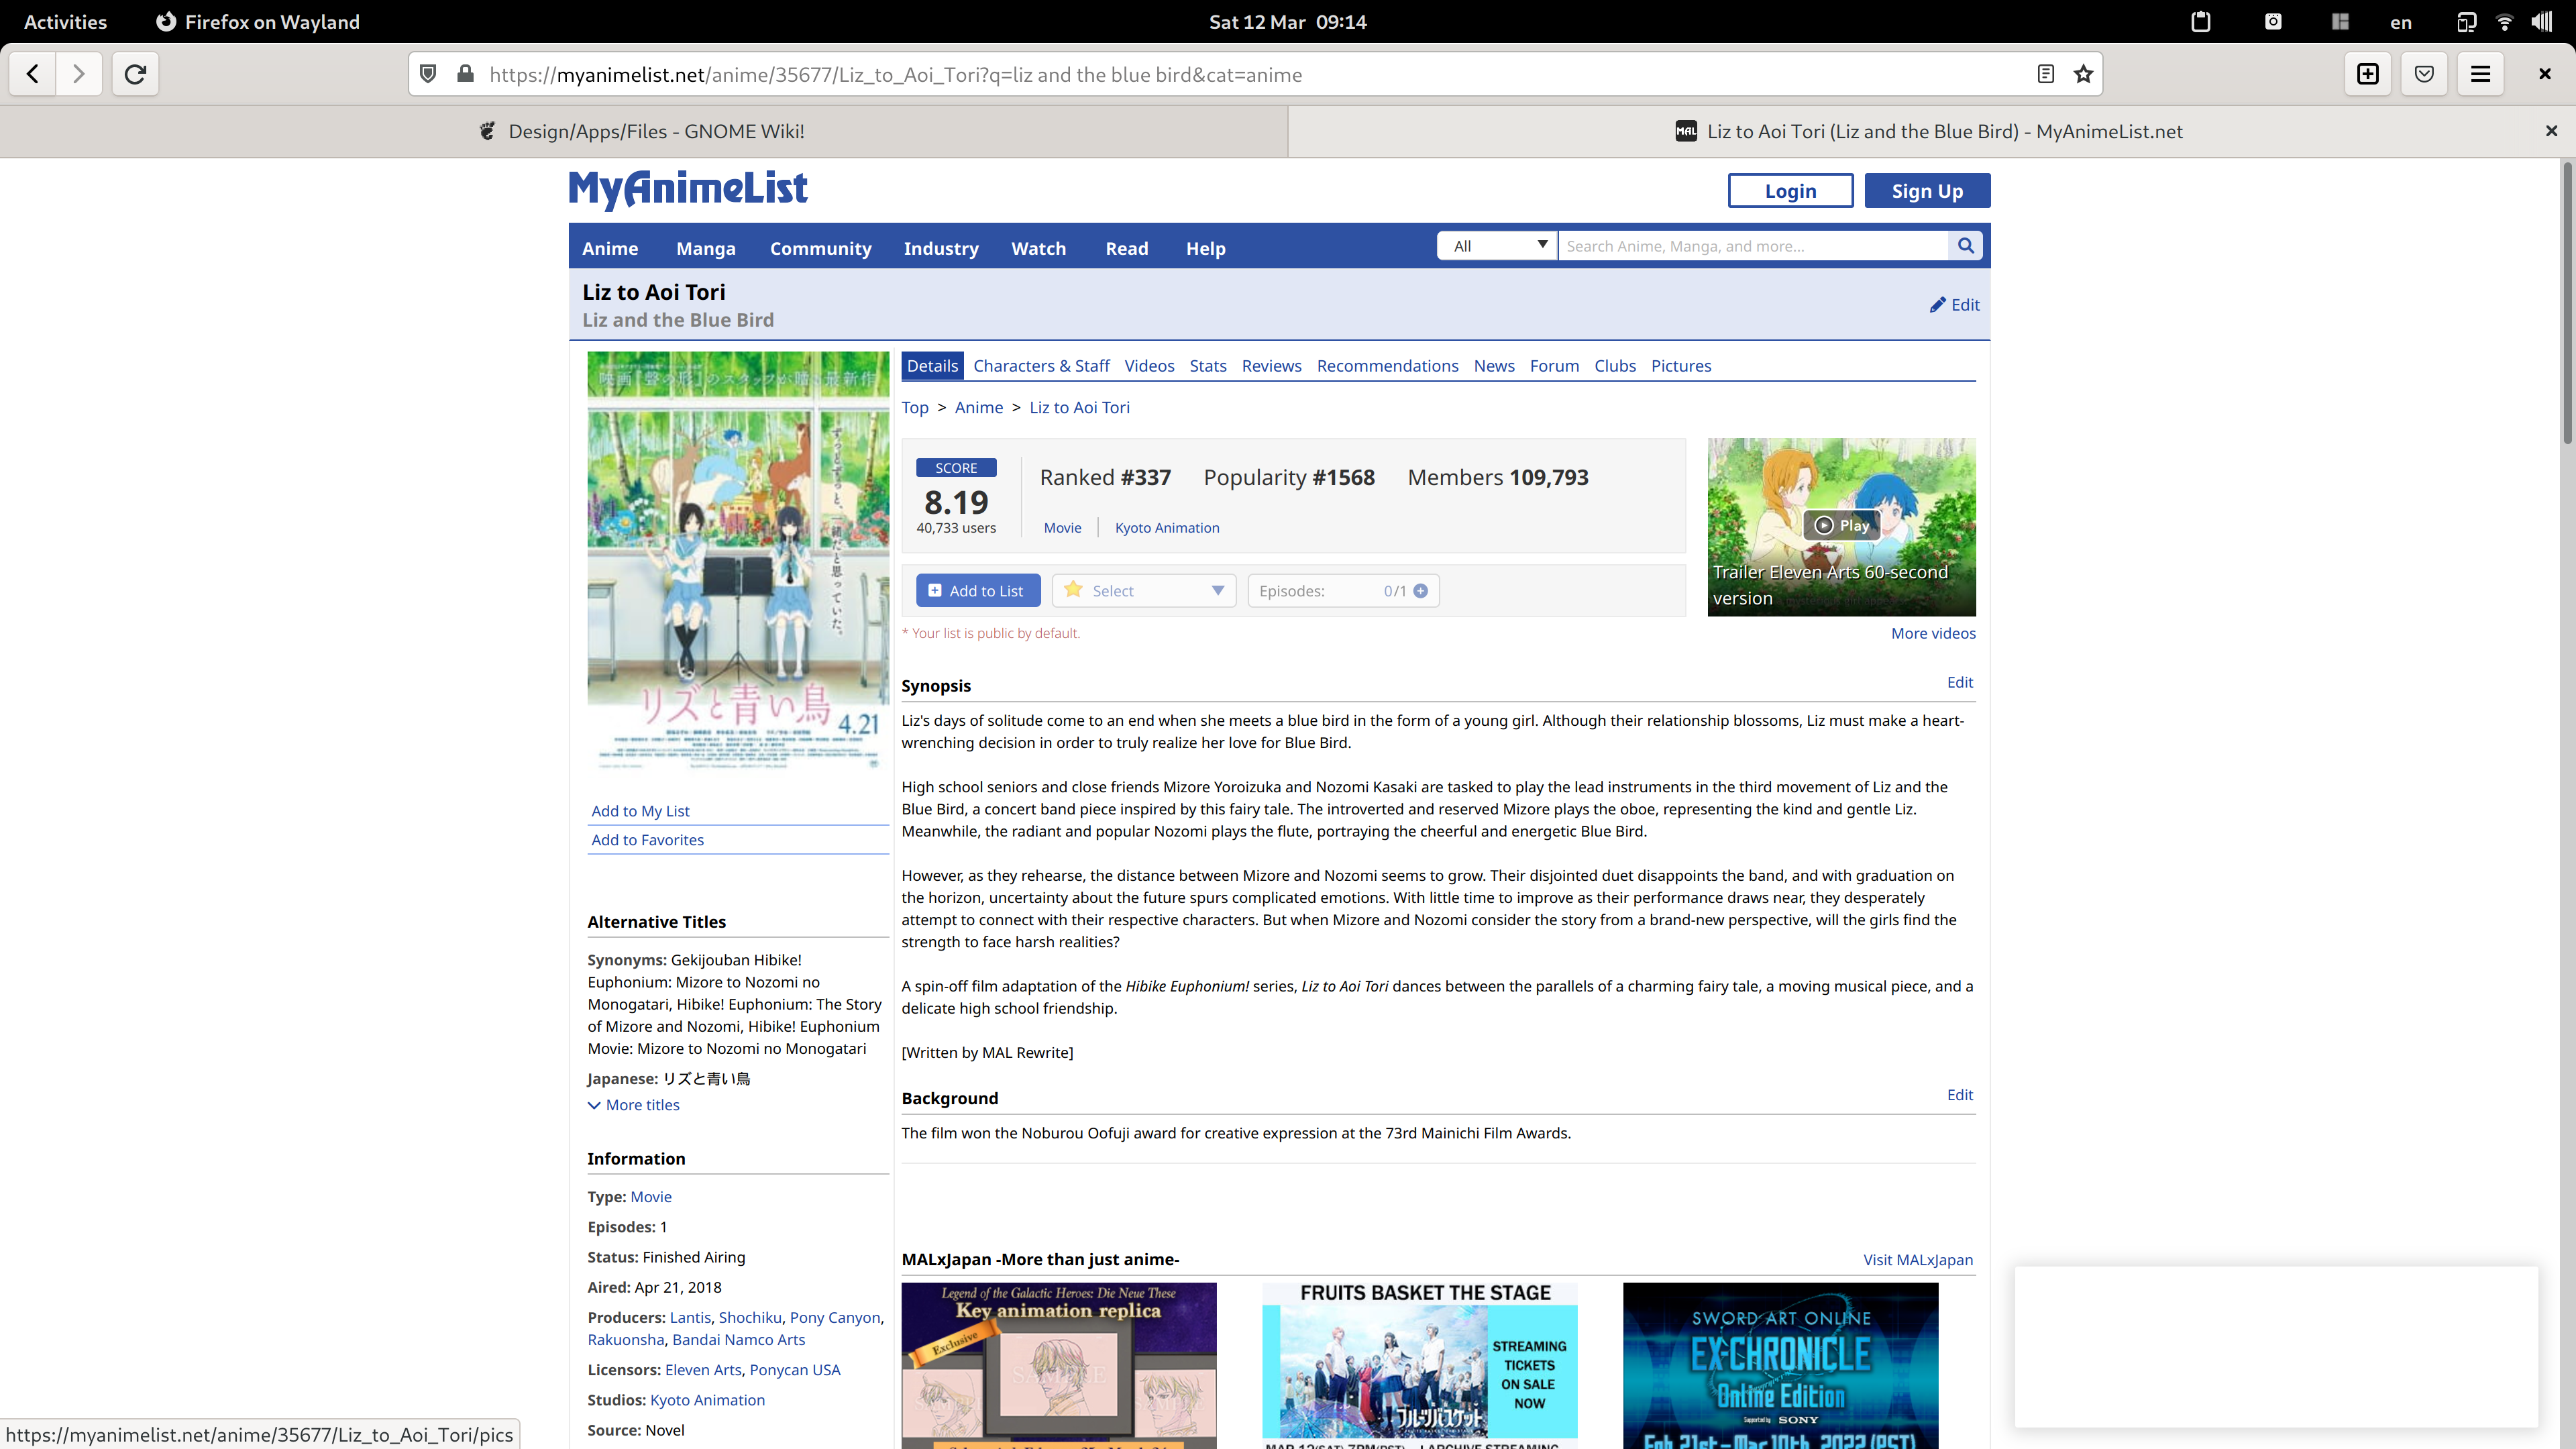
\includegraphics[width=\textwidth]{MAL.png}
\subsection{AniList}
\includegraphics[width=\textwidth]{aniList.png}
\subsection{Kitsu}
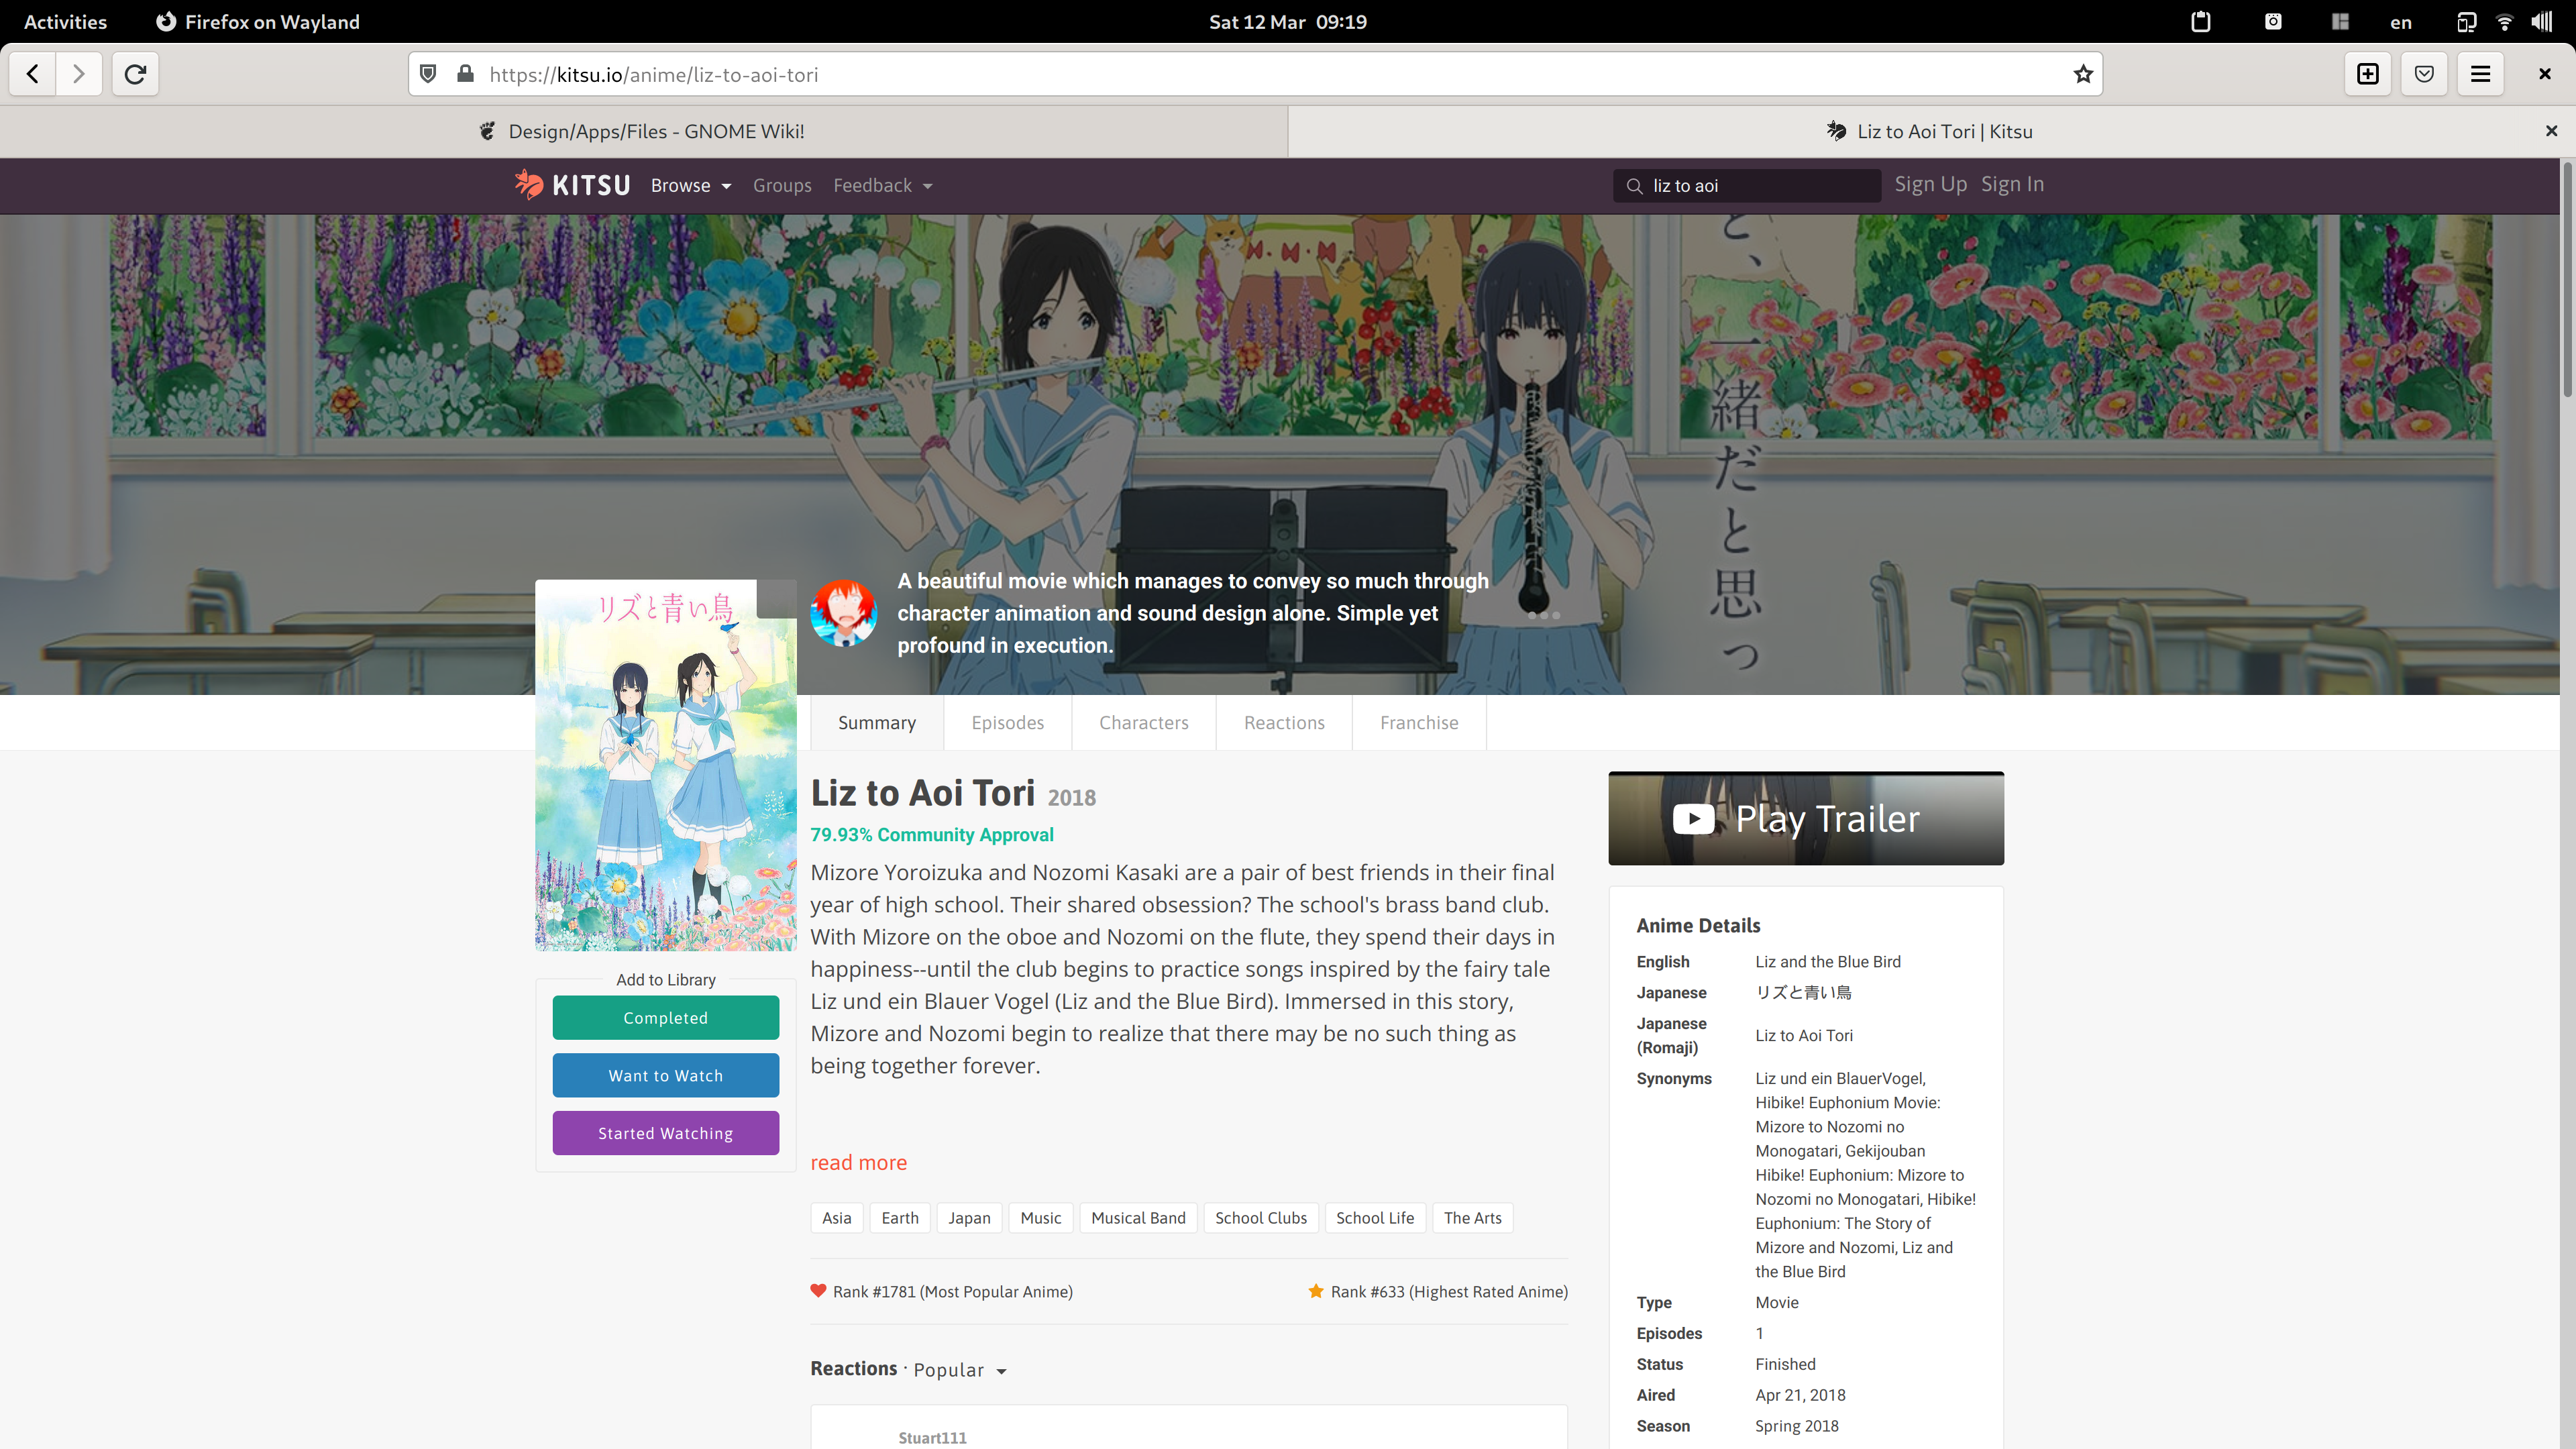
\includegraphics[width=\textwidth]{Kitsu.png}
\subsection{Anime Planet}
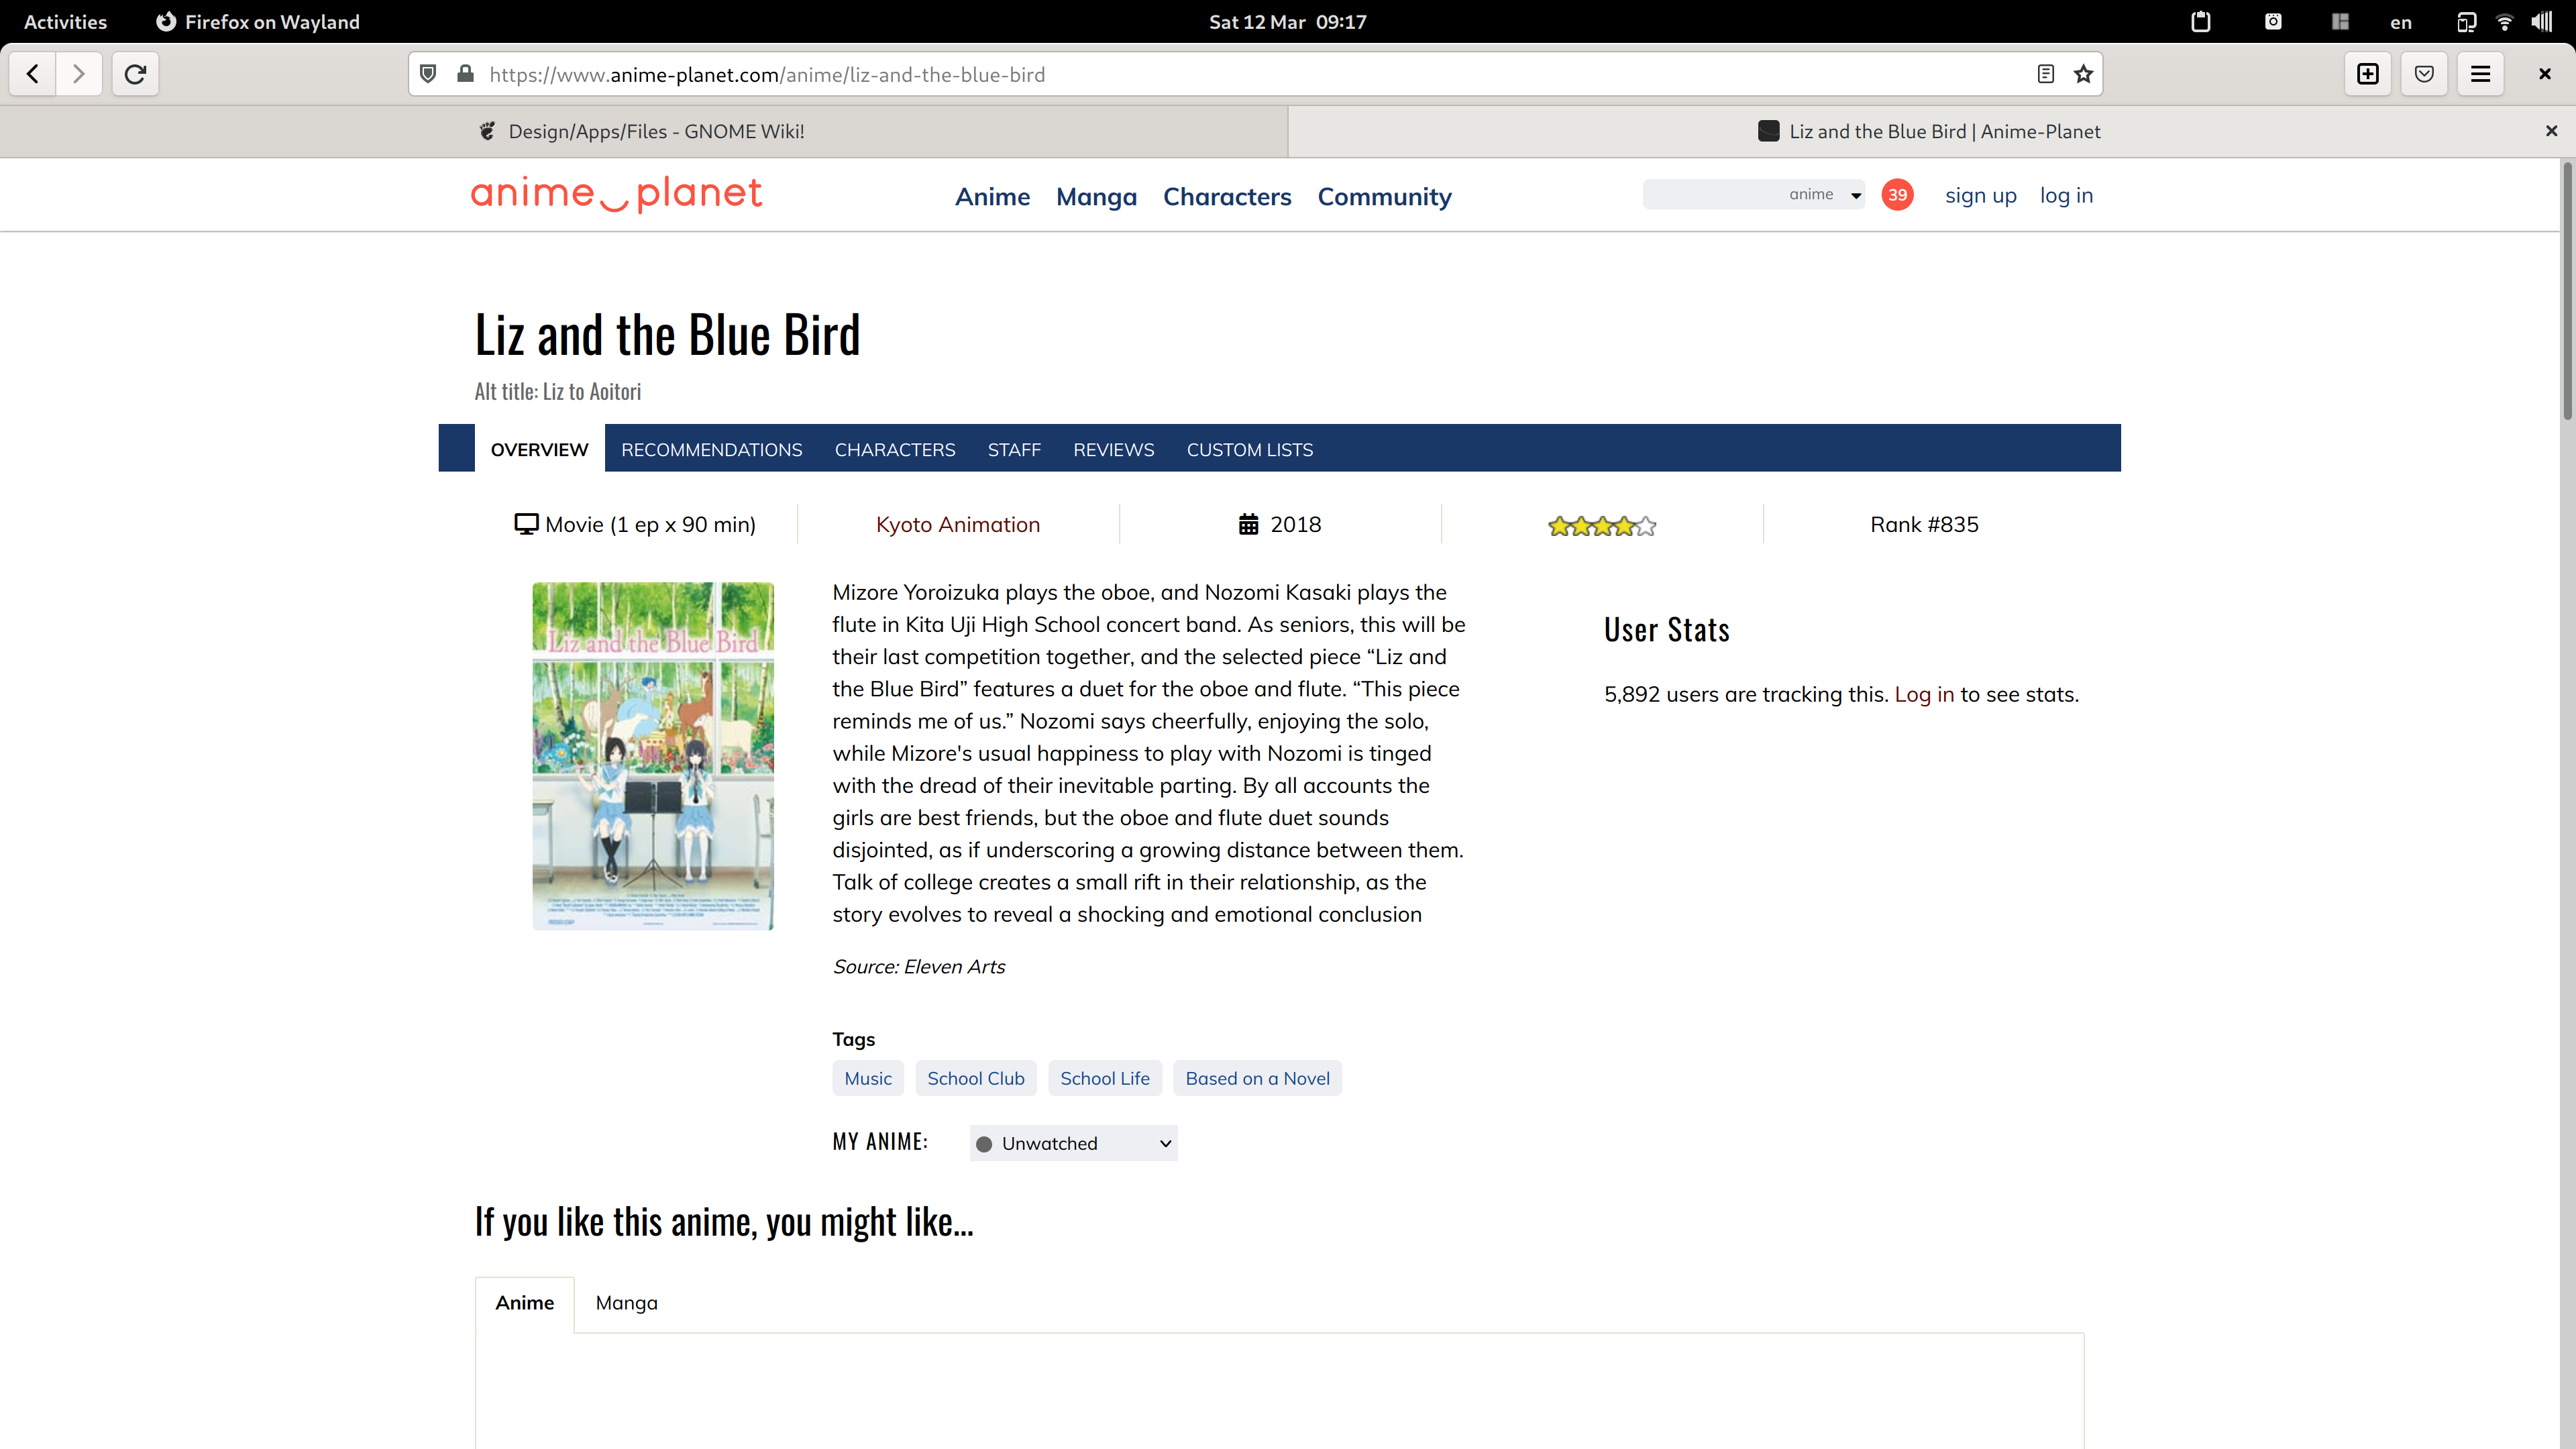
\includegraphics[width=\textwidth]{AP.png}
\subsection{AniDB}
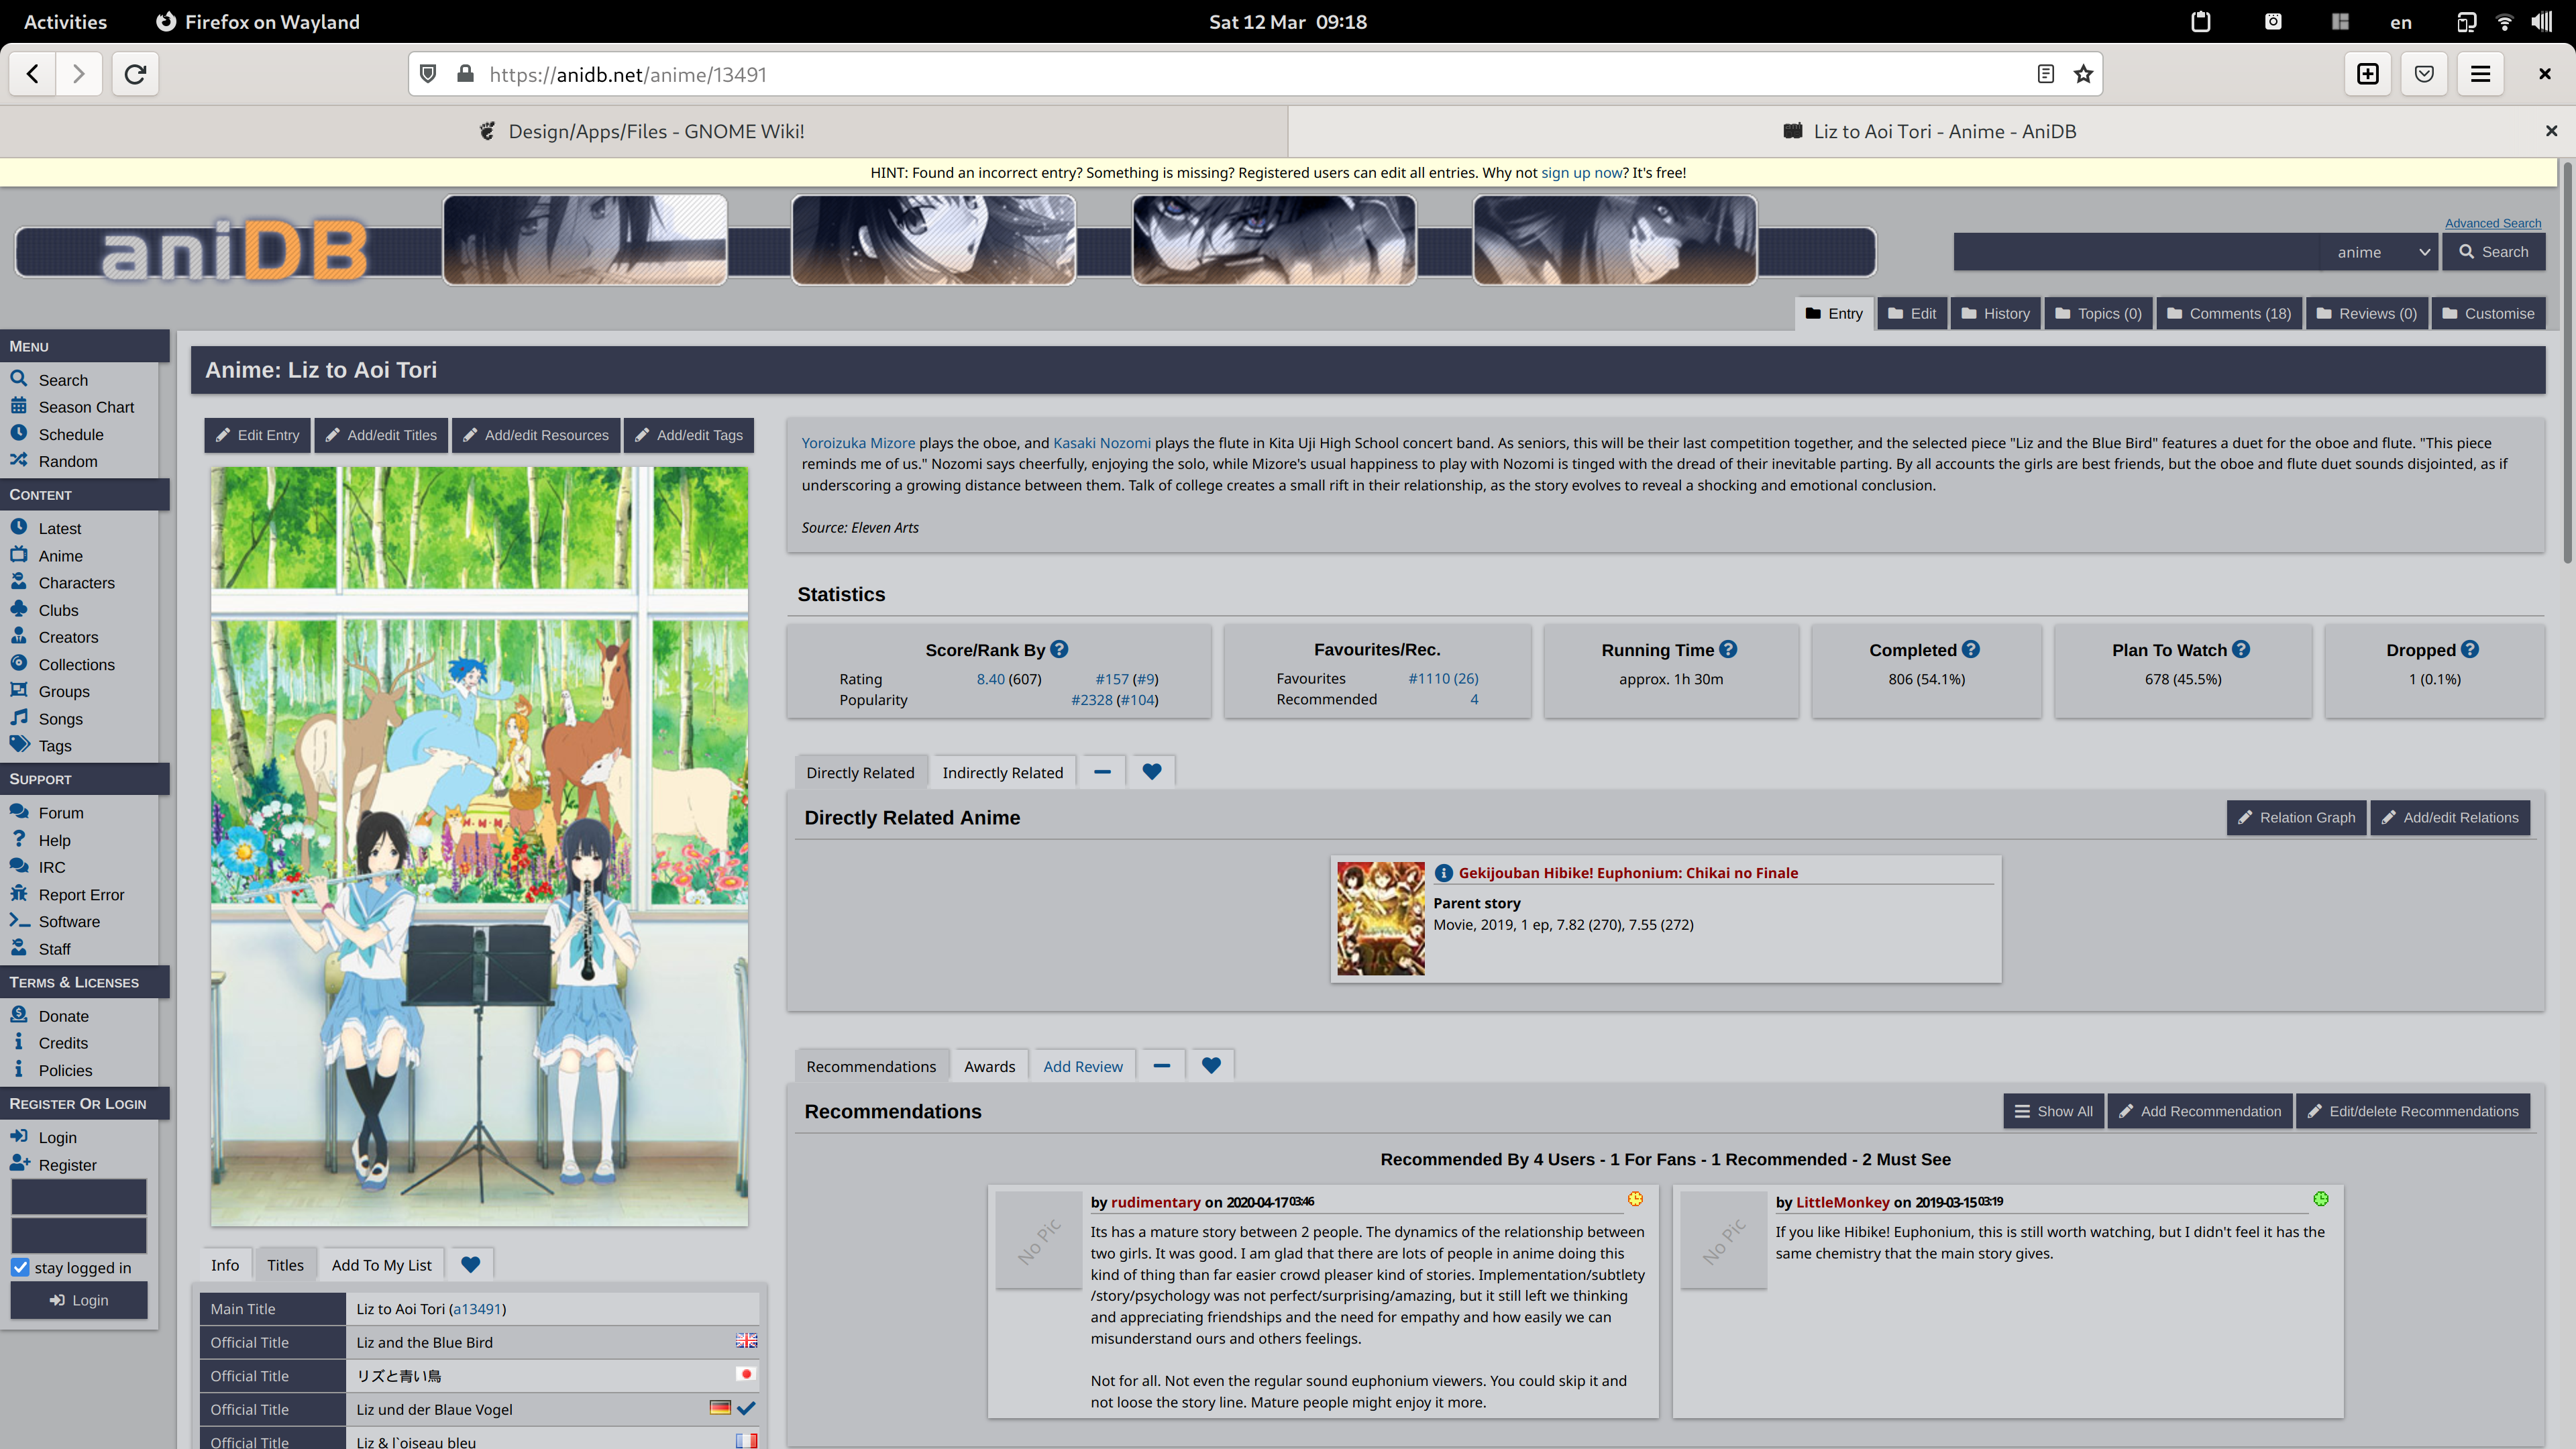
\includegraphics[width=\textwidth]{aniDB.png}

\end{document}